\chapter{Diseño de la aplicación}

En este capítulo veremos el diseño de la aplicación y qué tecnologías se han utilizado para su implementación.\\

La aplicación consiste en una página SPA (Single-Page Application) que obtiene datos de la página de la Liga de Fútbol Profesional, e interactúa con un cliente AngularJS a través de una API REST.\\

Alguna de las características de la aplicación son:

\begin{itemize}
\item Visualización de estadísticas de todos los equipos de la liga BBVA durante sus temporadas en primera división. Algunas de estas estadísticas son el número de temporadas en primera división, número de goles como local y visitante, número de partidos ganados, empatados y perdidos, porcentaje de victorias, derrotas y empates, y número de partidos según el resultado.

\item Visualización de estadísticas de todas las temporadas de la Liga BBVA, desde la temporada 1928-1929, de la competitividad (grafo evolutivo y medidas de competitividad).

\item Posibilidad de subir tus propios rankings para que pueda ser visualizado como un grafo de competitividad y calcular las medidas de competitividad asociados esos rankings subidos por el usuario.
\end{itemize}

\section{Arquitectura de la aplicación}

La arquitectura de la aplicación se puede ver en la Figura~\ref{fig:arquitectura}. Se puede observar que se trata de una arquitectura cliente-servidor. En la parte del servidor o backend, se encuentra el módulo de extracción de datos (parser) y la API REST. El primero de ellos, se encarga de extraer datos de la página oficial de Liga de Fútbol Profesional~\cite{lfp} y los guarda en la base de datos MySQL; y el segundo, es una API REST que permite extraer y obtener datos de la base de datos y comunicarse con el lado del cliente o frontend. En la parte del frontend, se encuentra la aplicación AngularJS, que se encarga de dar al usuario una interfaz gráfica con la que intercambiar datos a través de la API REST.

\begin{figure}[htb]
\centering
\arquitectura
\caption{Arquitectura de la aplicación}
\label{fig:arquitectura}
\end{figure}

\section{Tecnologías utilizadas}

Para implementar la aplicación anterior, se han utilizado distintas tecnologías, tanto en el lado del cliente como del servidor. A continuación, detallamos cada una de ellas distinguiendo si se han utilizado en un lado o en otro.

\subsection{Tecnologías del lado del servidor}

En el lado del servidor se han utilizado las siguientes tecnologías:

\begin{itemize}
\item Servidor HTTP Apache
\item MySQL
\item PHP
\item Composer
\item Slim Framework
\end{itemize}

\subsubsection*{Servidor HTTP Apache}

Apache~\cite{apache} es un servidor web HTTP de código libre disponible para todas las plataformas (Windows, Mac y Linux). Algunas de sus ventajas frente a sus competidores es su modularidad, su facilidad de uso y la gran comunidad de la que dispone por lo que existe una gran cantidad de información y documentación sobre este servidor. Además, es el servidor web más usado del mundo.

\begin{figure}[tbh]
\centering
\label{fig:apache}

\includegraphics[width=0.5\textwidth]{imagenes/apache}
\caption{Servidor HTTP Apache}
\end{figure}

\subsubsection*{MySQL}

MySQL~\cite{mysql} es un sistema de gestión de base de datos relacional. Se caracteriza por soportar un gran subconjunto del lenguaje SQL, es multiplataforma y permite la utilización de una gran cantidad de motores en cada tabla, tales como MyISAM, InnoDB, MySQL Cluster, etc.

\begin{figure}[tbh]
\centering
\label{fig:mysql}

\includegraphics[width=0.5\textwidth]{imagenes/MySQL}
\caption{MySQL}
\end{figure}

\subsubsection*{PHP}

PHP~\cite{php} es un lenguaje de programación de código abierto que puede ser usado tanto como lenguaje de scripting como lenguaje para el desarrollo web. PHP tiene tipado dinámico, es multiplataforma y permite trabajar con gran cantidad de sistemas de bases de datos como MySQL, Oracle, PosgreSQL, etc.

\begin{figure}[tbh]
\centering
\label{fig:php}

\includegraphics[width=0.5\textwidth]{imagenes/PHP}
\caption{PHP}
\end{figure}

\subsubsection*{Composer}

Composer~\cite{composer} es un sistema de gestión de paquetes PHP que permite descargar los proyectos y las dependencias de un proyecto, sin saber de cuáles se trata específicamente.

\begin{figure}[tbh]
\centering
\label{fig:composer}

\includegraphics[width=0.2\textwidth]{imagenes/composer}
\caption{Composer}
\end{figure}

\subsubsection*{Slim Framework}

Slim Framework~\cite{slim} es un micro framework de PHP que permite realizar aplicaciones web y APIs REST de una forma muy sencilla. Slim permite trabajar con rutas, sesiones y tiene soporte para HTTP, por lo que es capaz de manipular estados de las peticiones y respuestas, cabeceras, URIs, entre otros.

\begin{figure}[tbh]
\centering
\label{fig:slim}

\includegraphics[width=0.2\textwidth]{imagenes/slim}
\caption{Slim Framework}
\end{figure}

\subsection{Tecnologías del lado del cliente}

En el lado del cliente se han utilizado las siguientes tecnologías:

\begin{itemize}
\item HTML5
\item CSS3
\item JavaScript
\item Bower
\item Bootstrap
\item AngularJS
\item Cytoscape.js
\end{itemize}

\subsubsection*{HTML5}

HTML~\cite{html5} es un lenguaje de marcas que permite la construcción de páginas web. Su última versión, la versión 5, tiene importantes novedades con respecto a las versiones anteriores:

\begin{itemize}
\item Introducción de elementos semánticos
\item Introducción de atributos de control como números, fechas, calendarios, rangos, horas, ...
\item Introducción de elementos gráficos
\item Introducción de nuevas APIs como la de geolocalización, la de arrastrar y soltar, almacenamiento local, ...
\end{itemize}

\begin{figure}[tbh]
\centering
\label{fig:html5}

\includegraphics[width=0.2\textwidth]{imagenes/html5}
\caption{HTML5}
\end{figure}

\subsubsection*{CSS3}
CSS~\cite{css3} es un lenguaje usado para crear la vista de presentación de una página web, típicamente HTML o XML. La idea detrás de CSS es la de permitir separar la estructura de una página web de su presentación. Actualmente, se encuentra en la versión 3, llamada CSS3, aunque todavía no se encuentra finalizada en sus totalidad.

\begin{figure}[tbh]
\centering
\label{fig:css3}

\includegraphics[width=0.2\textwidth]{imagenes/css3}
\caption{CSS3}
\end{figure}

\subsubsection*{JavaScript}
Javascript~\cite{javascript} es un lenguaje de programación que permite dotar al HTML de animaciones, interactividad y efectos visuales dinámicos. También se puede usar en el lado del servidor. Es un lenguaje imperativo, débilmente tipado y dinámico y basado en prototipos.

\begin{figure}[tbh]
\centering
\label{fig:javascript}

\includegraphics[width=0.2\textwidth]{imagenes/javascript}
\caption{JavaScript}
\end{figure}

\subsubsection*{Bower}
Bower~\cite{bower} es un gestor de paquetes JavaScript. Se encarga de manejar las dependencias de un determinado paquete, descargándolas de forma transparente para el desarrollador. Es el análogo a Composer, pero para paquetes escritos en JavaScript.

\begin{figure}[tbh]
\centering
\label{fig:bower}

\includegraphics[width=0.3\textwidth]{imagenes/bower}
\caption{Bower}
\end{figure}

\subsubsection*{Bootstrap}
Bootstrap~\cite{bootstrap} es un framework CSS que permite desarrollar de forma fácil una aplicación web. Cuenta con multitud de componentes gráficos ya predefinidos como iconos, botones, barras de navegación, etiquetas, barras de progreso, barras de paginación, etc.

\begin{figure}[tbh]
\centering
\label{fig:bootstrap}

\includegraphics[width=0.7\textwidth]{imagenes/bootstrap}
\caption{Bootstrap}
\end{figure}

\subsubsection*{AngularJS}
AngularJS~\cite{angular} es un framework JavaScript para la creación de aplicaciones web SPA, mantenido y desarrollado por Google. Una aplicación SPA (Single-Page Application) es una aplicación web que ``simula'' ser una aplicación de escritorio, es decir, con sola una página.

\begin{figure}[tbh]
\centering
\label{fig:angular}

\includegraphics[width=0.3\textwidth]{imagenes/angular}
\caption{AngularJS}
\end{figure}

\subsubsection*{Cytoscape.js}

Cytoscape.js~\cite{cytoscape} es una librería JavaScript para el análisis y visualización de grafos.

\begin{figure}[tbh]
\centering
\label{fig:cytoscape}

\includegraphics[width=0.3\textwidth]{imagenes/cytoscape}
\caption{Cytoscape.js}
\end{figure}

\section{Backend}

En la Figura~\ref{fig:arquitectura} se puede observar que el backend está compuesto por una API REST y un parser para obtener los datos necesarios. Todos los datos se guardan en una base de datos relacional MySQL.

\subsection*{Parser}

El parser es un módulo que se encarga de obtener los datos de la liga BBVA, de todas las jornadas de forma automática. Es un módulo realizado en PHP, junto con la librería PHP Simple HTML DOM Parser. Esta librería simplifica la tarea de analizar el DOM de la página de la LFP, con la intención de que sea lo más fácil posible obtener los datos que necesitamos. Los datos que obtiene este parser son el histórico de partidos y rankings (clasificaciones con equipo, puntos, partidos ganados, partidos perdidos y partidos empatados, goles a favor y goles en contra) desde la primera temporada que se disputó, la 1928-1929.\\

Este módulo se compone de varios scripts PHP, donde cada uno de los ellos se encarga de realizar una tarea:

\begin{itemize}
\item \textbf{calendario.php}: es el script que se encarga de conocer el día en que finalizan todas las jornadas de la liga BBVA. Una vez que se tienen todas las fechas, se genera un archivo de texto, que se guarda en el \texttt{crontab}, para que el sistema se conecte y descargue los resultados de la página de forma automática. Se encuentra configurado para que se conecte todas las jornadas a las 4:00h del día siguiente que acaba una jornada.\\
Este es el único script que no es autónomo por sí mismo ya que es necesario, una vez al inicio de temporada, volver a ejecutarlo o incluso tener que reescribirlo para que vuelva a cargar los datos en el \texttt{crontab}.

\item \textbf{historico.php}: es el script que se encarga de descargar desde la página de la LFP el histórico de resultados desde la temporada 1928-1929. Se guardan en base de datos se guardan los nombres de los equipos y los goles a favor y en contra de cada equipo.

\item \textbf{rankings\_historicos.php}: es el script encargado de guardar las clasificaciones y los resultados históricos de la liga BBVA. En la clasificación guarda goles a favor, goles en contra, equipos, posición del equipo, puntos, partidos ganados, empatados y perdidos, diferencia de goles y la jornada de esa clasificación.

\item \textbf{equipos.php}: es el script encargado de guardar en base de datos todos los equipos de los que se dispone información.

\item \textbf{jornada\_actual.php}: es el script encargado de descargar los resultados de la jornada actual, y construir, a partir de los datos de base de datos, la clasificación de la jornada actual y guardarla en base de datos.

\end{itemize}

Todos los datos recogidos por los scripts anteriores, se guardan en tres tablas distintas:

\begin{itemize}
\item \textbf{Partidos}: es la tabla donde se guardan los resultados de cada uno de los partidos con los nombres de los equipos, jornada, goles local y los goles de cada uno de ellos.

\item \textbf{Rankings}: tabla donde se guardan las clasificaciones de todas las jornadas. Se incluyen datos como posición del equipo, número de puntos, número de partidos jugados, empatados y perdidos, goles a favor y goles en contra, y diferencia de goles.

\item \textbf{Equipos}: tabla donde se guardan los equipos junto a su nombre.
\end{itemize}

La Figura~\ref{fig:er-parser} muestra el diagrama Entidad-Relación completo del parser.

\begin{figure}[htb]
\centering
\erparser
\caption{Diagrama E-R asociado al parser}
\label{fig:er-parser}
\end{figure}

\clearpage

\subsection*{API REST}

REST (Representational State Transfer) es una arquitectura para el desarrollo de aplicaciones web. Se basa totalmente en HTTP, por lo que puede ser usado por cualquier dispositivo que entienda el protocolo HTTP.\\

REST tiene cuatro niveles según el modelo de madurez de Richardson~\cite{richardson}:

\begin{itemize}
\item El nivel 0 consiste en utilizar HTTP como método de transporte para llamadas remotas, pero sin utilizar ningún otro método de la web.

\item El nivel 1 es la introducción de recursos. Un recurso es la información a la que queremos acceder independientemente del formato en el que esté almacenado. Cada recurso debe tener una URI única.

\item El nivel 2 es el uso de los verbos HTTP. Cuando trabajamos con REST, podemos utilizar los verbos que vienen con HTTP como GET (consultar y leer recursos), POST (crear recursos), PUT (editar recursos), DELETE (borrar recursos), PATCH (editar partes concretas de un recurso). También se deben utilizar algunos de los códigos de estado de HTTP. Una lista de los estados de HTTP se pueden consultar en \cite{http-status}.

\item El nivel 3 es el uso de Hypermedia, cuyo objetivo es conectar mediante vínculos las aplicaciones cliente con las API. Se añade información adicional al recurso sobre su conexión con otro recursos conectados a él.
\end{itemize}

\begin{figure}[htb]
\centering
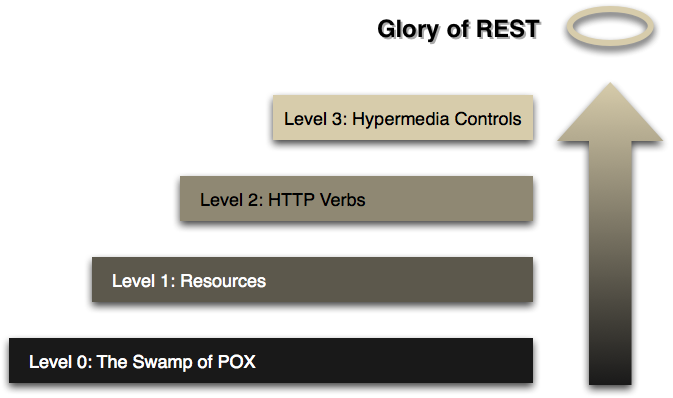
\includegraphics[width=0.6\textwidth]{imagenes/rest-levels}
\caption{Niveles de madurez de una API REST}
\label{fig:niveles-api-rest}
\end{figure}

Nuestra API REST sólo consta de los 3 primeros niveles del modelo de madurez de Richardson. Está implementada en PHP con el framework Slim, que es muy útil cuando se quieren implementar APIs de forma rápida y sencilla. Para el intercambio de datos entre el cliente y el servidor utilizamos el formato JSON (JavaScript Object Notation) que es muy ligero y de gran uso en el intercambio de información vía API REST.\\

Como en el parser, la API REST también hace uso de la base de datos, por lo que también tiene un modelo de datos asociada a ella. Consta de las mismas tablas que en caso del parser, más tres tablas más: User, Competitivity\_graph y Graph\_vertex.

\begin{itemize}
\item \textbf{User}: es la tabla encargada de mantener información de sobre los usuarios que están usando la API REST para subir sus propios rankings y calcular las medidas de competitividad asociadas a esos rankings. Guarda información de el nombre de usuario, la contraseña (cifrada con SHA1), el email, y el apiKey (código alfanumérico que sirve para identificar a un usuario de forma única en la aplicación. Se usa porque REST no tiene estado y es una forma de identificar a los usuarios).

\item \textbf{Competitivity\_graph}: es la tabla que guarda el nombre y las medidas de competitividad asociadas a un grafo de competitividad evolutivo. Las medidas que guarda son el grado medio normalizado (nmd), la fuerza media normalizada (nmd), la eficiencia, la longitud del camino característico (cpl), la tau de Kendall generalizada y el diámetro del grafo.

\item \textbf{Graph\_vertex}: es la tabla que guarda el conjunto de aristas del grafo de competitividad evolutivo. De cada arista se guarda el nodo origen, el destino y el peso de cada arista.
\end{itemize}

El diagrama Entidad-Relación asociado a la API REST se puede ver en la Figura~\ref{fig:er-api}.\\

El diseño completo de la API REST implementada se pueden ver en el Anexo~\ref{app:api-rest}.

\begin{figure}[htb]
\centering
\erapi
\caption{Diagrama E-R asociado a la API REST}
\label{fig:er-api}
\end{figure}


\section{Frontend}

El frontend consiste en una aplicación SPA implementada en AngularJS que se comunica con la API REST comentada anteriormente.\\

La aplicación depende de una serie de módulos Angular que permite una mayor interactividad con el usuario:

\begin{itemize}
\item \textbf{Angular-route}: módulo que permite la definición de nuevas rutas dentro de la aplicación Angular.

\item \textbf{Restangular}: módulo que permite hacer peticiones REST a un servidor.

\item \textbf{Angular-loading-bar}: módulo que permite añadir una barra de carga que indica si una página ha terminado de cargar.

\item \textbf{Angular-chart}: módulo que permite la representación de gráficos. Los tipos de gráficos que soporta son: gráfico de líneas, de radar, de barras y de sectores.

\item \textbf{Cytoscape.js}: módulo que permite representar y analizar grafos.
\end{itemize}

\subsection{Vista de la aplicación}

En esta sección, veremos el aspecto global de la aplicación y las vistas de las que consta ésta.\\

La página de inicio se puede ver en la Figura~\ref{fig:inicio-aplicacion}. En la parte superior, hay una barra de navegación desde la que puede iniciar sesión. En la parte lateral izquierda, se muestran todas las temporadas desde la 1928-1929, hasta la temporada actual y todos los equipos que han jugado en primera división en la Liga. La parte que falta de la pantalla muestra las estadísticas de la temporada actual: clasificación, el histórico de posiciones a lo largo de las jornadas, el grafo de competitividad y distintas medidas de competitividad en forma de gráfico.\\


\begin{figure}[htb]
\centering
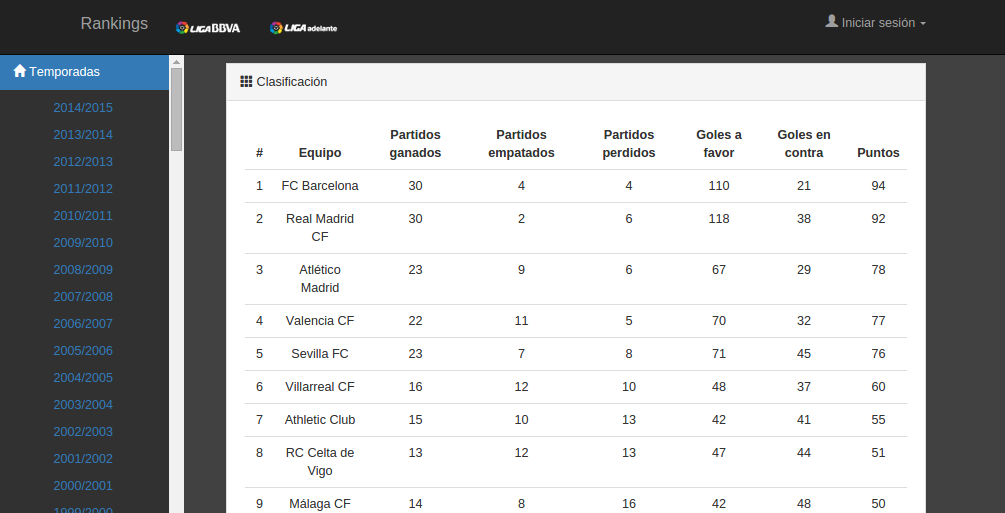
\includegraphics[width=0.9\textwidth]{imagenes/pantallazos-aplicacion/inicio}
\caption{Inicio de la aplicación}
\label{fig:inicio-aplicacion}
\end{figure}

El histórico de posiciones (Figura~\ref{fig:inicio-historico}) muestra, mediante un gráfico de líneas, la posición de cada equipo durante todas las jornadas. Se pueden ver los cambios de posiciones de cada equipo, y las tendencias que siguen a lo largo de la temporada.\\


\begin{figure}[htb]
\centering
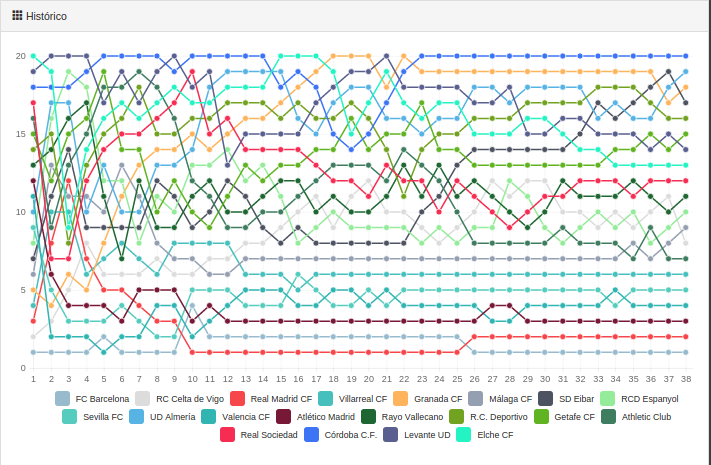
\includegraphics[width=0.9\textwidth]{imagenes/pantallazos-aplicacion/inicio-historico}
\caption{Histórico de posiciones durante la temporada}
\label{fig:inicio-historico}
\end{figure}

Las medidas de competitividad (Figura~\ref{fig:medidas}) se muestran en dos gráficos distintos: el primero de ellos, muestra un gráfico de radar con seis medidas de competitividad (fuerza  y grado medio normalizado, eficiencia, diámetro, longitud del camino característico y tau de Kendall generalizada); en el segundo se muestran las distribuciones acumuladas de la fuerza y del grado normalizado.\\

\begin{figure}[htbp]
\centering
\subfigure[Medidas de competitividad en un gráfico de radar]{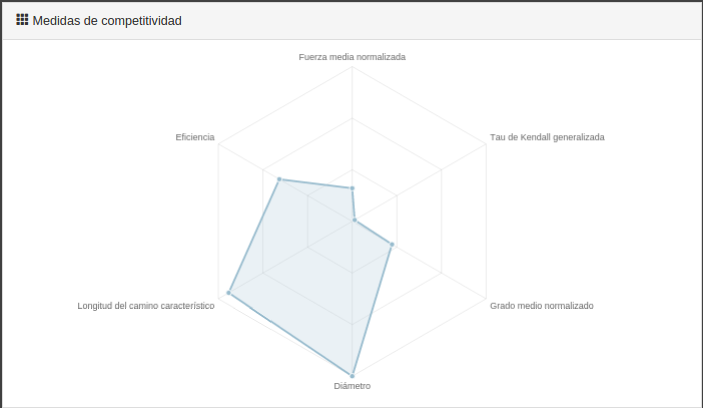
\includegraphics[width=0.45\textwidth]{imagenes/pantallazos-aplicacion/inicio-medidas1}}
\subfigure[Medidas de competitividad en un gráfico de líneas]{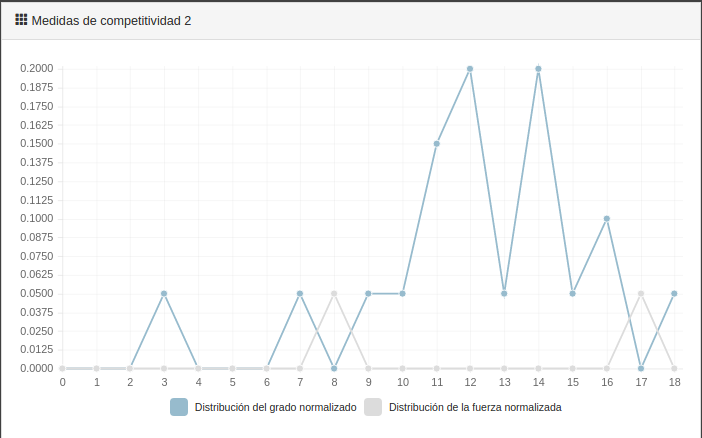
\includegraphics[width=0.45\textwidth]{imagenes/pantallazos-aplicacion/inicio-medidas2}}
\caption{Gráficos con las medidas de competitividad} \label{fig:medidas}
\end{figure}

Por último, en la pantalla de inicio/temporada, se muestra el grafo de competitividad evolutivo (Figura~\ref{fig:inicio-grafo}). Se muestra el grafo junto con los nombres de los equipos, y sus respectivos escudos.\\


\begin{figure}[htb]
\centering
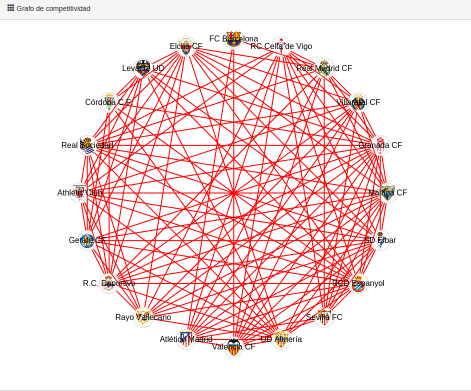
\includegraphics[width=0.9\textwidth]{imagenes/pantallazos-aplicacion/inicio-grafo}
\caption{Grafo de competitividad en la aplicación}
\label{fig:inicio-grafo}
\end{figure}

De la misma forma, si pinchamos sobre un equipo en la pantalla de inicio/temporada nos mostrará información relativa a ese equipo, como escudo y distintas estadísticas. \\

Las primeras estadísticas que se muestran son las relativas al histórico, como goles totales, número de victorias, derrotas y empates, número de temporadas en primera división. Todas estas estadísticas se dan tanto para equipo local como visitante (Figura~\ref{fig:equipo-estadisticas}).\\

\begin{figure}[htb]
\centering
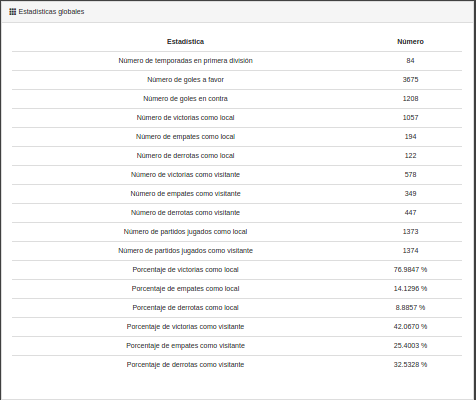
\includegraphics[width=0.9\textwidth]{imagenes/pantallazos-aplicacion/equipo-estadisticas}
\caption{Estadísticas globales de un equipo}
\label{fig:equipo-estadisticas}
\end{figure}

Otras estadísticas que se muestran son los porcentajes de victorias, derrotas y empates tanto como de local como de visitante (Figura~\ref{fig:equipo-local}) en forma de gráfico circular. También se pueden ver los mismos gráficos, pero para goles (a favor y en contra) tanto como local como para visitante.\\

\begin{figure}[htb]
\centering
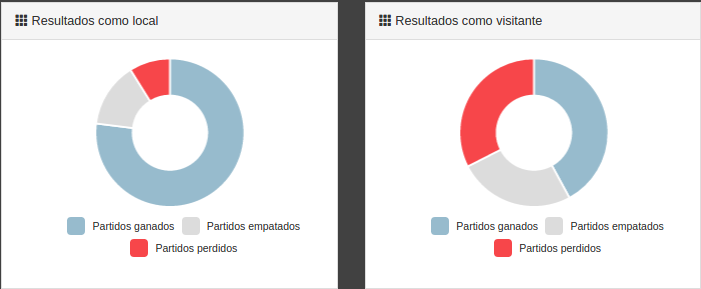
\includegraphics[width=0.9\textwidth]{imagenes/pantallazos-aplicacion/equipo-local}
\caption{Estadísticas de resultados de un equipo}
\label{fig:equipo-local}
\end{figure}

Por último, se muestran las estadísticas por resultados, es decir, se muestran el número de veces que el partido acabó 0-0, 1-0, etc. \\

\begin{figure}[htb]
\centering
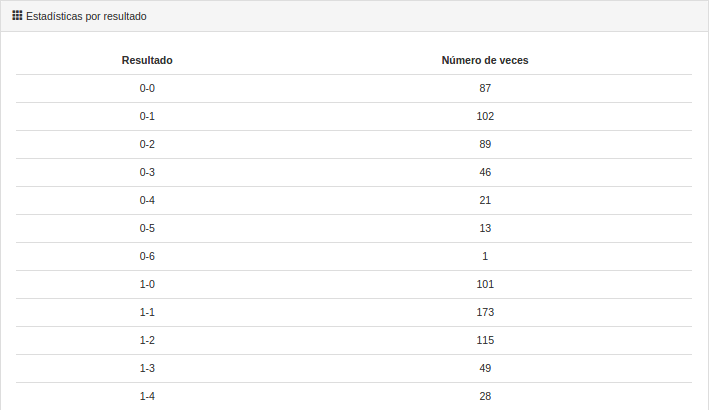
\includegraphics[width=0.9\textwidth]{imagenes/pantallazos-aplicacion/equipo-resultados}
\caption{Estadísticas por resultados de un equipo}
\label{fig:equipo-resultados}
\end{figure}

A parte de ver los resultados de la Liga, también se puede ver el gráfico de competitividad y las medidas para unos rankings de lo que disponga el usuario. Para ello, lo primero que deberá hacer el usuario será registrarse. Para hacerlo, debe ir a \emph{Iniciar Sesión} en la parte superior de la pantalla y pulsar sobre \emph{Registrarse}. Se mostrará un formulario de registro, en el que se deberán rellenar el nombre de usuario, la contraseña y el correo electrónico (Figura~\ref{fig:registro}).\\

\begin{figure}[htb]
\centering
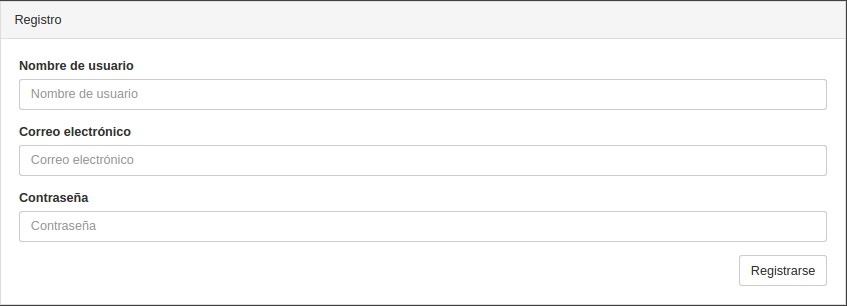
\includegraphics[width=0.9\textwidth]{imagenes/pantallazos-aplicacion/registro}
\caption{Formulario de registro}
\label{fig:registro}
\end{figure}

Una vez rellenos estos datos, nos redirigirá a una nueva página desde la que podremos iniciar sesión. Esta vez sólo nos pedirá el usuario y la contraseña (Figura~\ref{fig:inicio-sesion}). Una vez introducidos los datos de forma correcta, nos llevará a la página de perfil del usuario, en la que se indican todos los rankings que hemos subido.

\begin{figure}[htb]
\centering
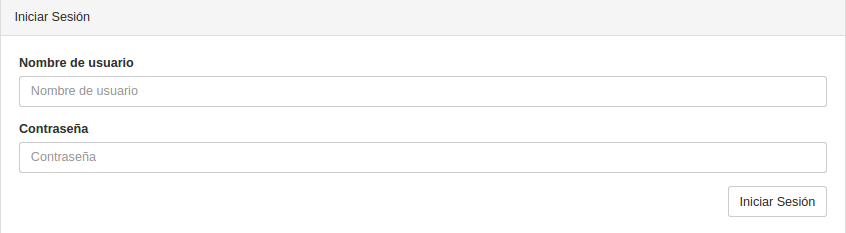
\includegraphics[width=0.9\textwidth]{imagenes/pantallazos-aplicacion/inicio-sesion}
\caption{Formulario para iniciar sesión}
\label{fig:inicio-sesion}
\end{figure}

Para añadir un nuevo ranking, deberemos hacer click sobre el botón \emph{+} que aparece en la parte superior derecha de la página de perfil. Nos mostrará un formulario en el que nos pedirá subir un archivo (Figura~\ref{fig:nuevo-ranking}). \\

\begin{figure}[htb]
\centering
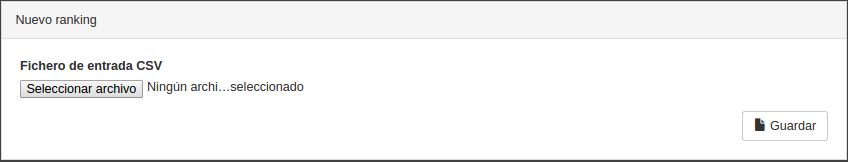
\includegraphics[width=0.9\textwidth]{imagenes/pantallazos-aplicacion/nuevo-ranking}
\caption{Formulario para añadir un nuevo ranking}
\label{fig:nuevo-ranking}
\end{figure}

El fichero que se suba debe tener el siguiente formato:

\begin{minted}{bash}
Nombre del grafo,4,4
RMA,BAR,SEV,VAL
BAR,SEV,VAL,RMA
RMA,BAR,VAL,SEV
RMA,VAL,BAR,SEV
\end{minted}

En la primera línea del archivo, se deben indicar el nombre que llevará ese grafo, el número de equipos y el número de jornadas. Todo ello separado por comas. A partir de la segunda línea hasta el número de jornadas, se deben indicar los nombres de los equipos de izquierda a derecha, donde la izquierda indica mayor posición en el ranking, y la derecha menor posición en el ranking. También deben ir separados por comas.\\

Una vez que se ha cargado el ranking, la aplicación volverá a la página de perfil, donde se mostrará el ranking que se acaba de insertar. Si pinchamos en el nombre de uno de los rankings que acabamos se subir se mostrará el grafo y las medidas de competitividad (Figura~\ref{fig:grafo-medida}). 

\begin{figure}[htbp]
\centering
\subfigure[Grafo de competitividad]{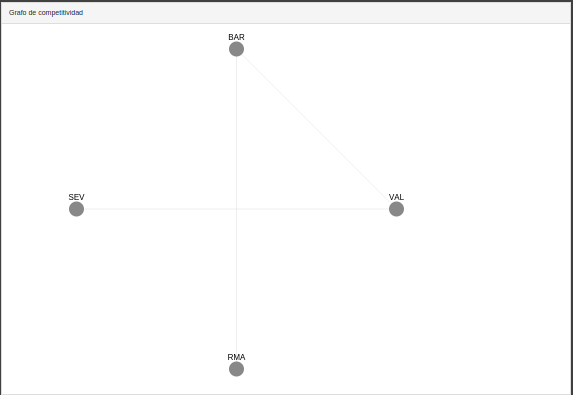
\includegraphics[width=0.9\textwidth]{imagenes/pantallazos-aplicacion/ver-grafo}}
\subfigure[Medidas de competitividad]{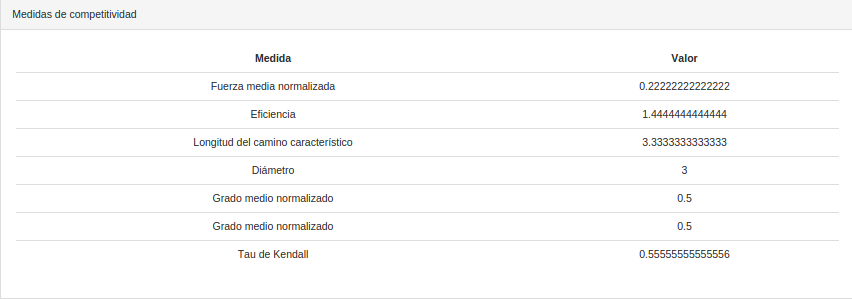
\includegraphics[width=0.9\textwidth]{imagenes/pantallazos-aplicacion/ver-medidas}}
\caption{Grafo y medidas de competitividad}
\label{fig:grafo-medidas}
\end{figure}
